%! TEX root = ../main.tex
\documentclass[../main.tex]{subfiles}
\begin{document}
\section{Verfahren}
\subsection{Selective Laser Melting}
Im Jahr 1995 wurde nun ein dem SLA ähnliches Verfahren entwickelt, das Selective-Laser-Melting-Verfahren. Bei diesem wird statt dem Üblichen Photosensitiven UV-Kunstharz und einem UV-LCD feinstes Metallgranulat mit einem herkömmlichen Laser verwendet, welcher dieses in einem Pulverbett zusammenschweißt und somit additive Herstellung ermöglicht. \parencite{3FAKTUR_1}
\begin{figure}[h]
\begin{center}
	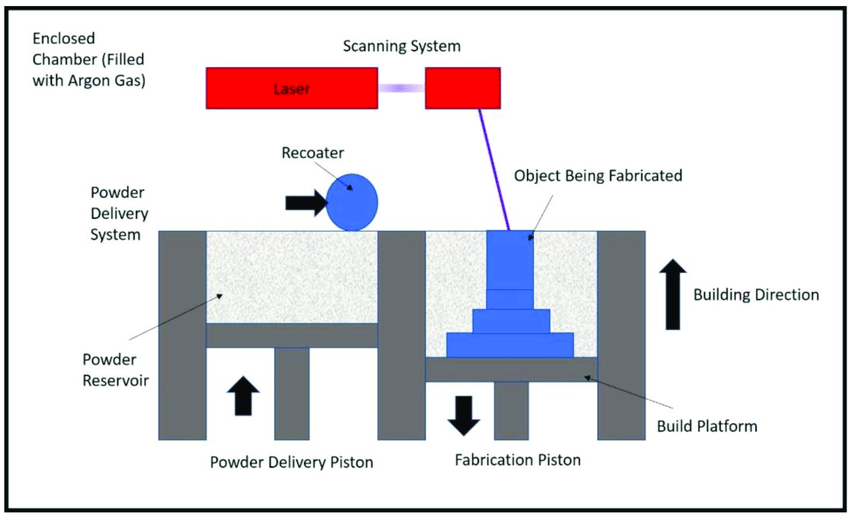
\includegraphics[width=.5\textwidth]{slm_diagram}
	\label{img:slm_diagram}
	\ccaption{Schematischer Aufbau einer SLM-Maschine}{\url{https://www.researchgate.net/publication/326891428/figure/fig1/AS:659597278855194@1534271654724/Schematic-diagram-of-the-selective-laser-melting-SLM-process.png}}
\end{center}
\end{figure}	
SLM ist ein Schichtverfahren, was daran erkennbar ist, dass es Schicht für Schicht ein Bauteil aufbaut. Dies passiert auf einer Bauplatform, welche nach jeder Schicht sich um die Schichtdicke nach unten bewegt, um das Auftragen einer neuen Schicht zu ermöglichen. 
Hinzu kommt, dass SLM ein Pulverbett-Verfahren ist, was wiederrum bedeutet, dass eine neue perfekt ebene Schicht auf dem Baustück aufgetragen werden muss nach jedem Absenken der Platform.
Hierfür ist ein Wiederbeschichtungswerkzeug vorhanden. Nach jeder Absenkung des Druckbettes wird über die Pulverlieferungsplatte Baumaterial nachgeliefert, welche dann vom Wiederbeschichtungswerkzeug eben verteilt wird am Druckbett. Der Exzess wird aufgefangen und gesiebt, um die Verschwendungsrate gering zu halten. 
Die Distanz des Wiederbeschichtungswerkzeugs zum Druckbett bestimmt die Schichtdicke, welche große Auswirkungen auf den Teil hat. Eine höhere Schichtdicke (über \qty{50}{\micro\meter}) führt zu schnellerer Produktionszeit, aber das produzierte Teil benötigt daraufhin mehr Nachbearbeitung durch verschiedene Verfahren wie Drehen, Polieren und Schleifen, um die korrekten Dimensionen zu garantieren.
Dennoch ist die Vielseitigkeit der Grund warum SLM sich so großer Beliebtheit erfreut. Mit verschiendenen Temperaturen des Lasers lassen sich viele Materialien verarbeiten, wie Fe-C-Stähle mit einem C-Gehalt von maximal \qty{0.3}{\percent}wt, Titan und Aluminium.

\end{document}
